\subsection{Ballmaschine (Eruieren der Nenndrehzahl)}

\begin{tabular}{p{3.6cm}p{9.4cm}}
\rule{0pt}{11pt}\textit{Typ}              & Ballmaschine \\ 
\rule{0pt}{11pt}\textit{Datum}:           & 06.11.2014   \\
\rule{0pt}{11pt}\textit{Ort}:             & Labor HSLU \\
\rule{0pt}{11pt}\textit{Tester}:          & Matteo, Yves, Pascal\\
\rule{0pt}{11pt}\textit{Ziel des Testes}: & Eruieren der Nenndrehzahl der DC-Motoren, Optimaler Wurfwinkel, Drehzahl der Schwungräder.  \\
\rule{0pt}{11pt}\textit{Fazit / Verbesserungs-\newline vorschlag}: & Die Ballzuführung muss automatisiert und gleichbleibend sein, damit genaue Aussagen über die Wurfweite gemacht werden können. 
Unterschiedliche Tennisballmarken haben unterschiedliche Eigenschaften betreffend Wurfweite -> Fünf Bälle der „richtigen“ Marke kaufen. \\
\end{tabular}
\begin{figure}[h!]
	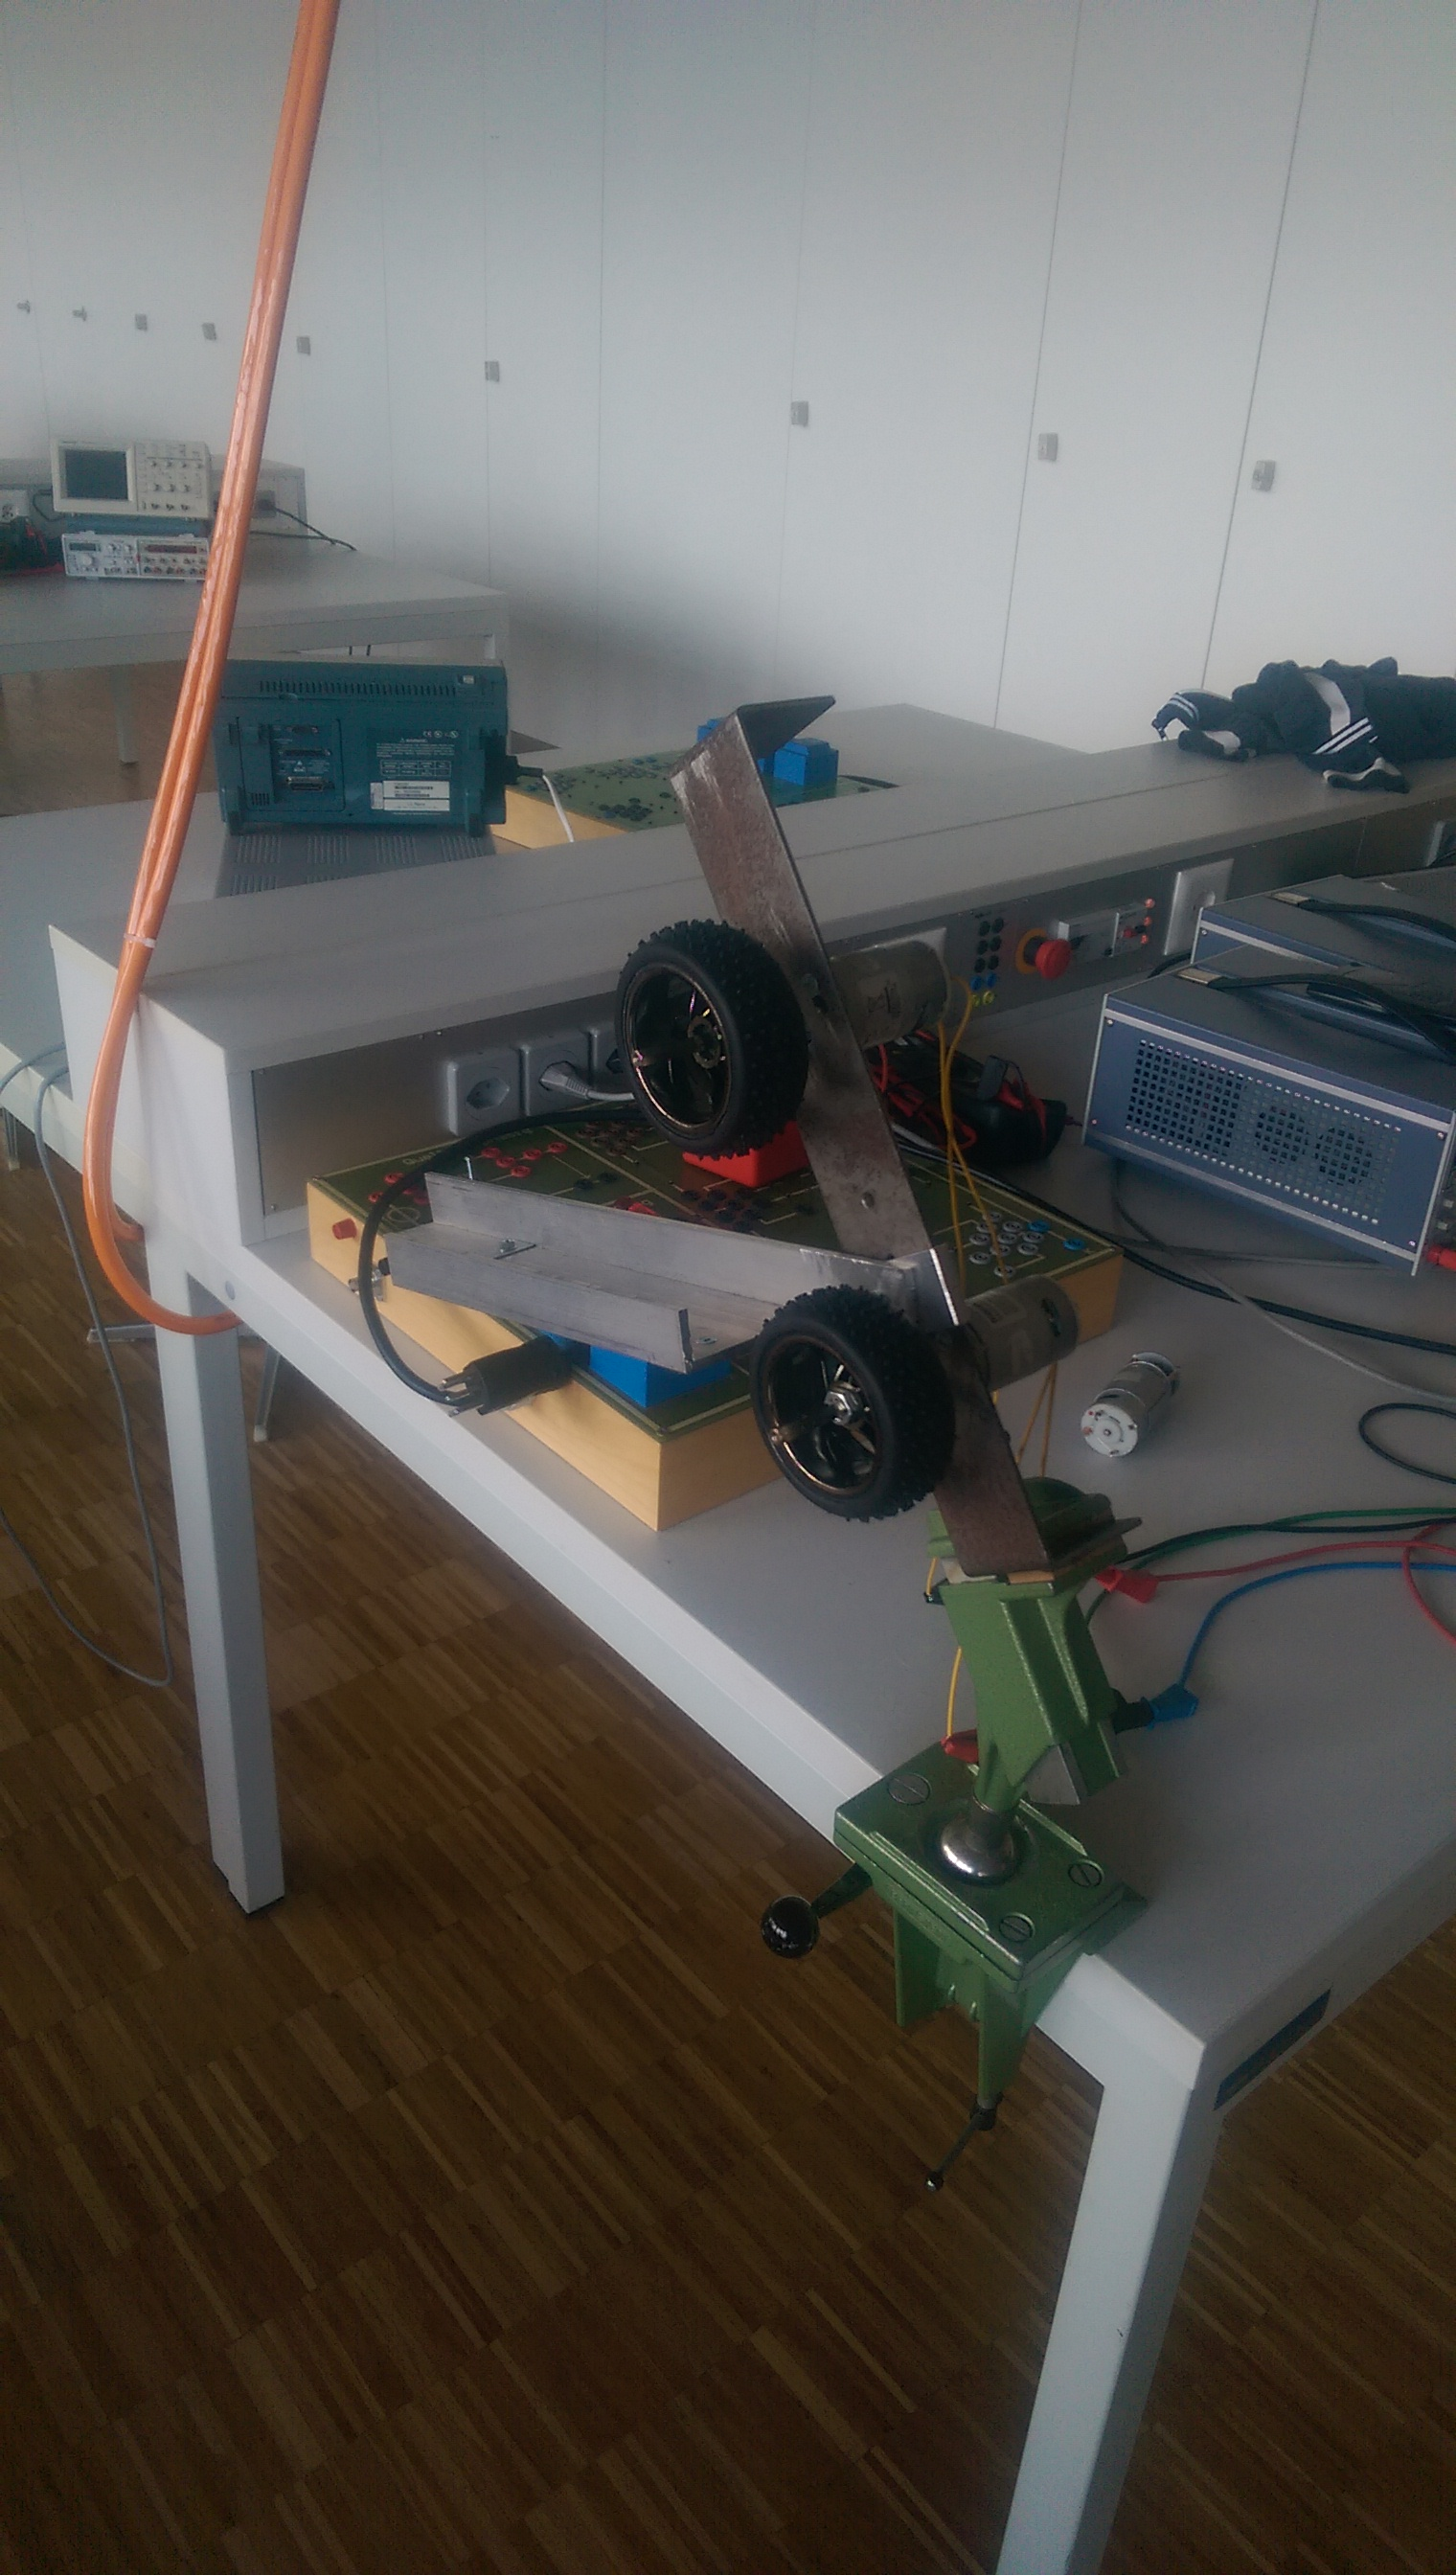
\includegraphics[width=0.7\textwidth,clip,trim=0mm 10cm 0mm 12cm]
	{Funktionstests/Bilder/Ballmaschine_Drehzahl1.jpg}
	\centering
	\caption{Funktionsmuster Ballmaschine} 
\label{abb:Ballmaschine_Drehzahl}
\end{figure}